\chapter{Installazione}
\label{Installazione}
\thispagestyle{plain}

%\section{Introduzione}
L'installazione di ShareLaTeX è stata fatta su una macchina virtuale ospitata da un server del laboratorio AImageLab. Tale macchina ha nome \verb|sharelatex| ed esegue il sistema operativo Ubuntu 18.04 LTS, il più recente alla data corrente. Il sistema è accessibile sia dall'interno dell'ateneo (se collegati alla rete locale), sia dall'esterno, grazie all'apertura della porta 443, all'indirizzo \url{sharelatex.ing.unimore.it}. L'installazione e la configurazione sono avvenute seguendo i passi sotto riportati. L'attuale amministratore del sistema è il Dott. Federico Bolelli.

\section{Docker}
Per il progetto ShareLaTeX si è optato per l'installazione di Docker CE, in quanto non risultano necessarie le funzionalità aggiuntive dell'Enterprise Edition, rivolte invece alle grandi imprese. L'installazione può avvenire in diversi modi, come indicato nella guida ufficiale \cite{docker_install}. Si è scelto di utilizzare il metodo raccomandato da Docker, ovvero tramite i loro repository.

\subsection{Download}
Aggiornare l'indice dei pacchetti di \verb|apt-get|:
\begin{lstlisting}
sudo apt-get update
\end{lstlisting}
Installare i pacchetti necessari per permettere a \verb|apt-get| di utilizzare un repository su HTTPS:
\begin{lstlisting}
sudo apt-get install \ 
    apt-transport-https \
    ca-certificates \
    curl \
    software-properties-common
\end{lstlisting}
Aggiungere la chiave GPG ufficiale di Docker:
\begin{lstlisting}
curl -fsSL https://download.docker.com/linux/ubuntu/gpg | sudo apt-key add -
\end{lstlisting}
Verificare di possedere la chiave con la fingerprint\\
\verb|9DC8 5822 9FC7 DD38 854A E2D8 8D81 803C 0EBF CD88|\\
confrontando gli ultimi 4 byte della fingerprint:
\begin{lstlisting}
sudo apt-key fingerprint 0EBFCD88
\end{lstlisting}
che dovrebbe produrre un output simile al seguente:
\begin{lstlisting}
pub   4096R/0EBFCD88 2017-02-22
Key fingerprint = 9DC8 5822 9FC7 DD38 854A E2D8 8D81 803C 0EBF CD88
uid     Docker Release (CE deb) <docker@docker.com>
sub     4096R/F273FCD8 2017-02-22
\end{lstlisting}
Montare il repository specificando l'architettura (in questo caso x64):
\begin{lstlisting}
sudo add-apt-repository \
"deb [arch=amd64] https://download.docker.com/linux/ubuntu \
$(lsb_release -cs) \
stable"
\end{lstlisting}

\subsection{Installazione}
Installare l'ultima versione di Docker CE:
\begin{lstlisting}
sudo apt-get install -y docker-ce
\end{lstlisting}
Verificare che Docker CE sia installato correttamente avviando l'immagine \verb|hello-world|:
\begin{lstlisting}
sudo docker run hello-world
\end{lstlisting}


\section{Docker Compose}
Docker Compose non è incluso all'interno di Docker CE. La sua installazione è necessaria ai fini del progetto per poter gestire i tre container che strutturano l'applicazione: ShareLaTeX, MongoDB e Redis.
\begin{figure}[h]
    \centering
    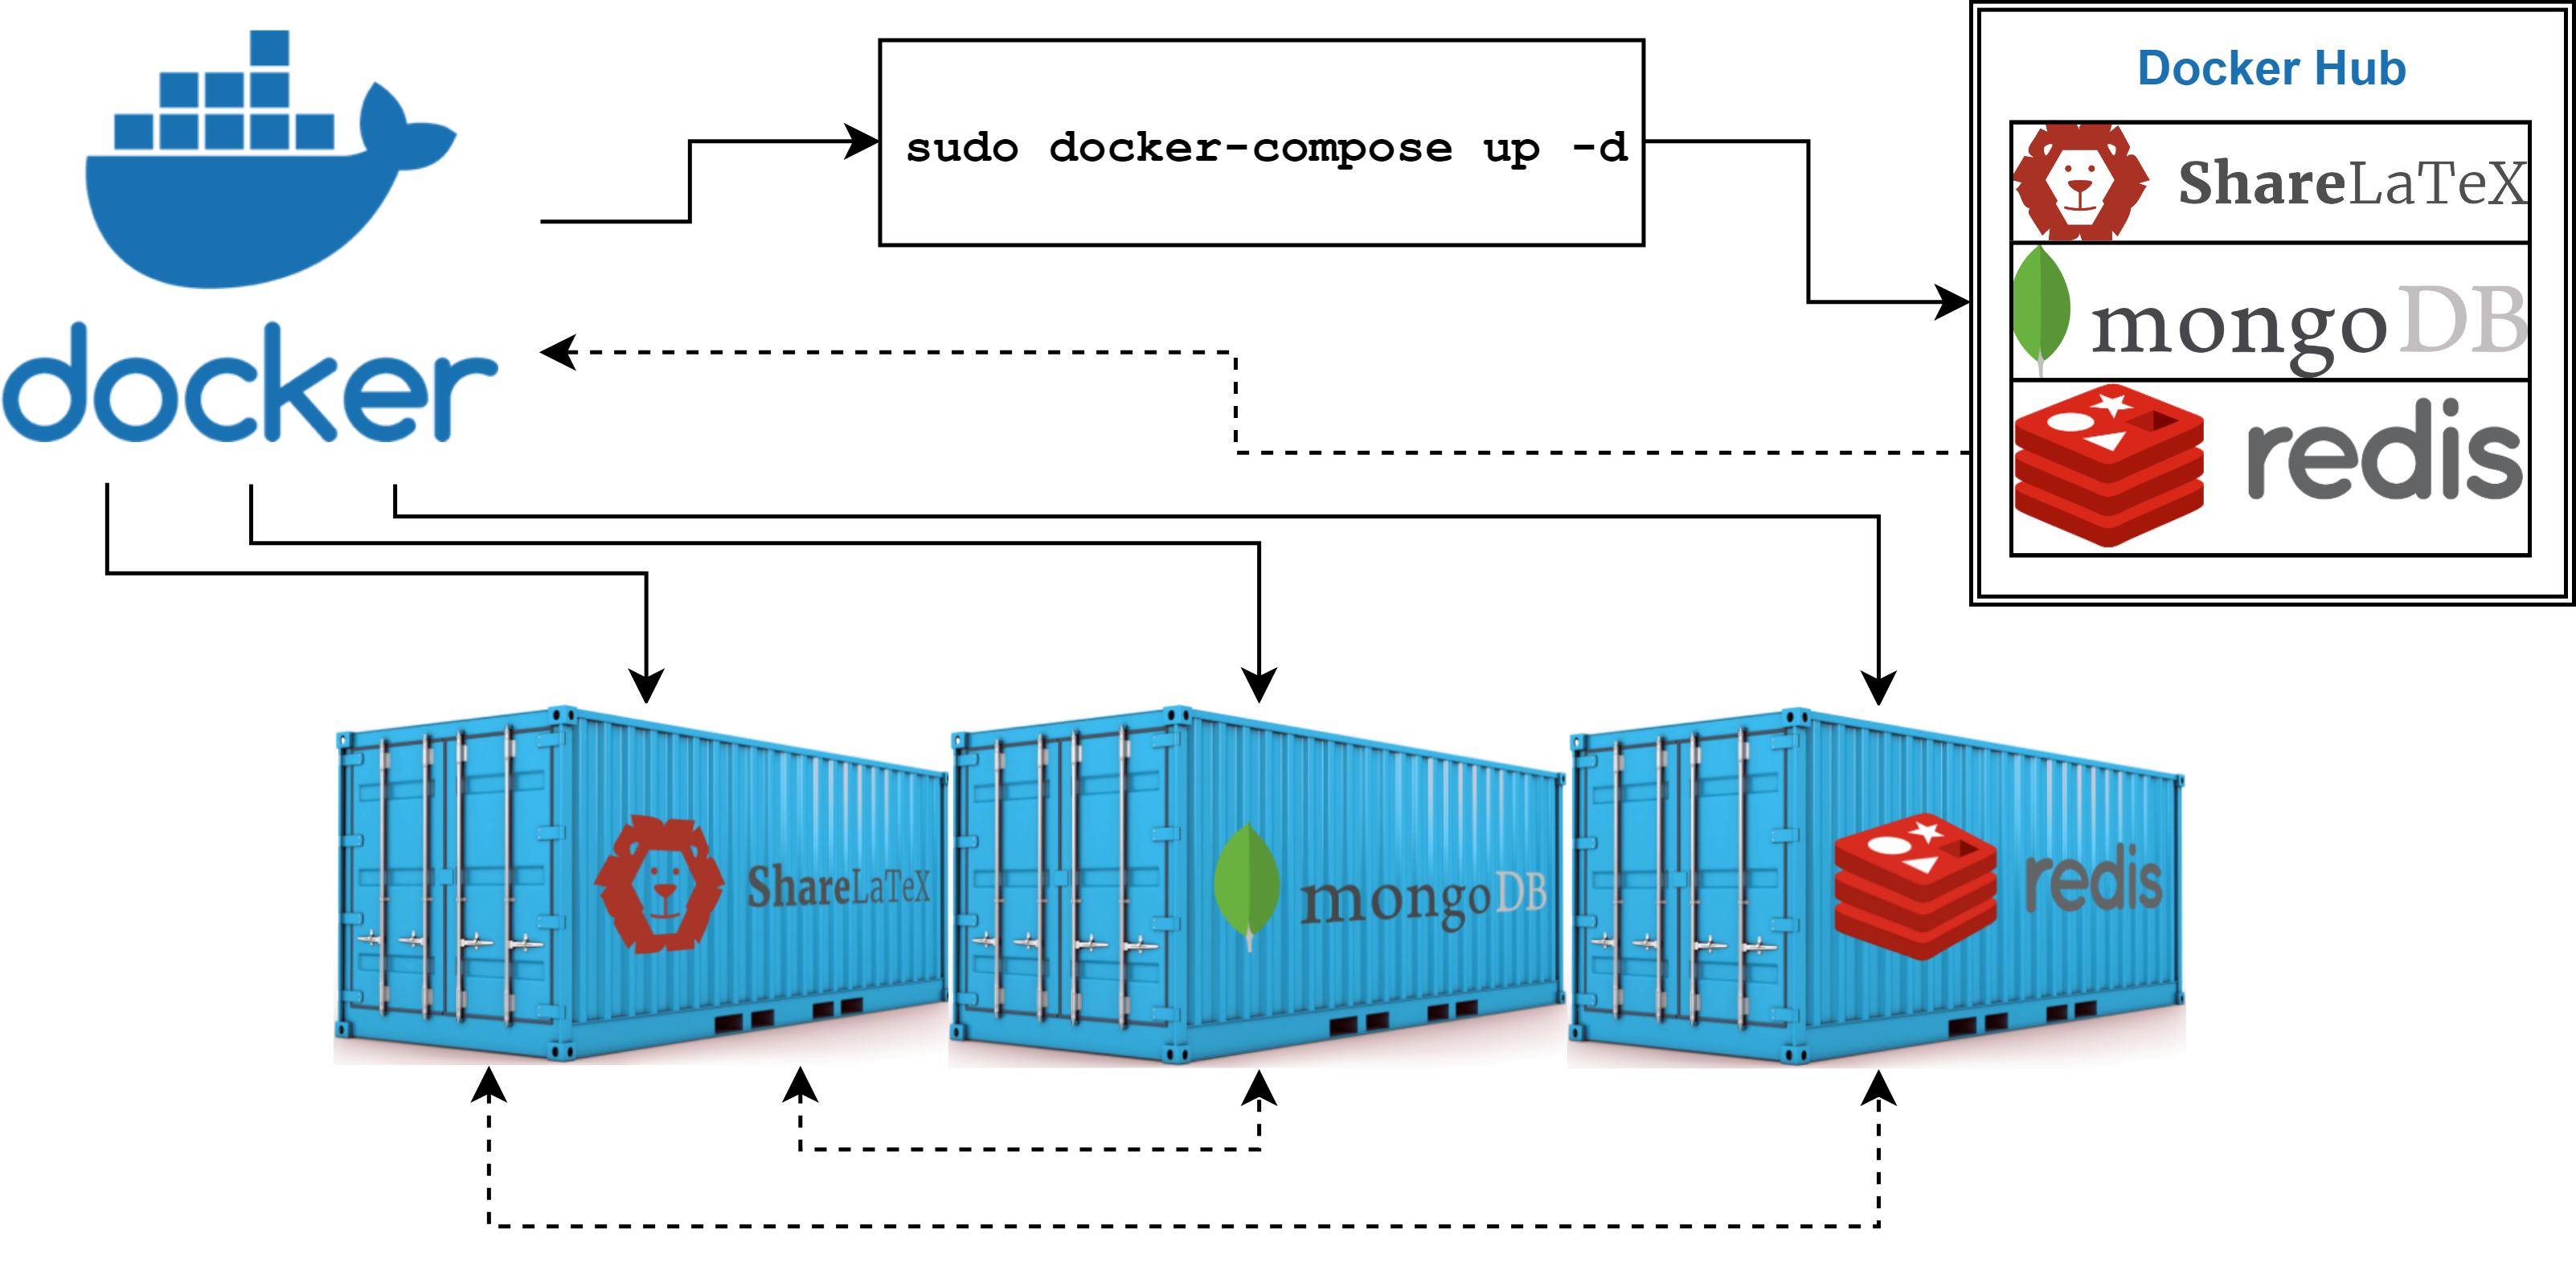
\includegraphics[width=\textwidth]{immagini/docker_container_dependencies.png}
    \caption{Esecuzione di Docker Compose e dipendenze fra container}
    \label{fig:docker_compose_dipendenze}
\end{figure}

\subsection{Download e installazione}
Con il comando che segue è possibile scaricare la versione 1.21.2 di Docker Compose. Per installare un'altra versione del software, eventualmente più aggiornata, è necessario modificare l'URL inserendo la versione richiesta. Per informazioni sull'ultima versione disponibile, visitare \verb|github.com/docker/compose/releases|.
\begin{lstlisting}
sudo curl -L https://github.com/docker/compose/releases/download/1.21.2/docker-compose-$(uname -s)-$(uname -m) -o /usr/local/bin/docker-compose
\end{lstlisting}
Occorre quindi applicare i permessi di esecuzione al file binario:
\begin{lstlisting}
sudo chmod +x /usr/local/bin/docker-compose
\end{lstlisting}
e testare l'installazione:
\begin{lstlisting}
docker-compose --version
\end{lstlisting}

\subsection{Configurazione}
Creare una directory dal nome \verb|sharelatex| e inserirvi \verb|docker-compose.yml|. Il template fornito dagli sviluppatori di ShareLaTeX per l'installazione tramite Docker è il seguente:
\lstinputlisting[caption={Template di docker-compose.yml}, captionpos=b, label=code:docker-compose.yml]{script/docker-compose-ridotto.yml}
Oltre a creare il container di ShareLaTeX, il file configura MongoDB e Redis. Inoltre fornisce una buona interfaccia per fornire impostazioni a ShareLaTeX\footnote{Approfondimento nel capitolo \hyperref[Configurazione]{\enquote*{Configurazione}}.}.
\begin{lstlisting}
mkdir sharelatex
cd sharelatex
wget https://raw.githubusercontent.com/aimagelab/sharelatex/master/docker-compose.yml
\end{lstlisting}
Infine avviare i container di ShareLaTeX, MongoDB e Redis usando le impostazioni di \verb|docker-compose.yml|. L'opzione \verb|-d| serve per avviare i container in modalità \enquote*{detached}, ovvero in background.
\begin{lstlisting}
sudo docker-compose up -d
\end{lstlisting}
Per visualizzare i container attualmente attivi, eseguire il comando:
\begin{lstlisting}
sudo docker ps
\end{lstlisting}

\section{TeX Live}
TeX Live \cite{texlive} è un distribuzione del sistema \TeX ~per installare, gestire e aggiornare pacchetti utilizzati per scrivere in \LaTeX. L'installazione completa dei pacchetti di TeX Live è essenziale per poter utilizzare qualsiasi pacchetto all'interno dei propri documenti. La totalità dei pacchetti occupa molta memoria sul disco (circa 7 GB), pertanto l'immagine di ShareLaTeX in Docker Hub presenta solo un'installazione parziale di TeX Live. La procedura di installazione richiederà molto tempo (circa 2 ore). L'immagine utilizzata per il container ShareLaTeX contiene la versione 2017 di TeX Live. Per l'installazione completa dei pacchetti di TeX Live 2018 e la risoluzione dei conflitti dei pacchetti preinstallati versione 2017, si è seguita la guida di aggiornamento fornita da TeX Live \cite{texlive_upgrade}.

\subsection{Fasi preliminari}
Modificare la variabile d'ambiente \verb|PATH|. Il modo più efficace e persistente consiste nell'aggiunta di \verb|PATH| fra le variabili d'ambiente di ShareLaTeX in \verb|docker-compose.yml|:
\begin{lstlisting}
environment:
    PATH: /usr/local/sbin:/usr/local/bin:/usr/sbin:/usr/bin:/sbin:/bin:/usr/local/texlive/2018/bin/x86_64-linux
\end{lstlisting}
Si ricorda che il ripristino/ricreazione di un qualunque container eliminerà tutte le modifiche ad esso apportate. Ciò significa che un eventuale riavvio del container ShareLaTeX dopo l'installazione completa di TeX Live ripristinerebbe lo stato dell'installazione iniziale. Questo può succedere, ad esempio, a seguito di modifiche al file \verb|docker-compose.yml| e all'esecuzione di \verb|sudo docker-compose up -d|. Pertanto è opportuno montare un volume esterno in corrispondenza della directory \verb|/usr/local/texlive/2018| per rendere persistenti i file dell'aggiornamento:
\begin{lstlisting}
volumes:
    - ~/sharelatex_texlive:/usr/local/texlive/2018
\end{lstlisting}
Salvare quindi le modifiche e riavviare i container:
\begin{lstlisting}
sudo docker-compose up -d
\end{lstlisting}

\subsection{Aggiornamento}
Per eseguire l'aggiornamento è necessario avviare una bash all'interno del container ShareLaTeX. Docker permette di avviare comandi all'interno dei container mediante il comando \verb|exec|. Le opzioni \verb|-t| e \verb|-i| servono rispettivamente per creare una pseudo-TTY e per renderla interattiva:
\begin{lstlisting}
sudo docker exec -ti sharelatex bash
\end{lstlisting}
Una volta all'interno del container, visitare il percorso \verb|/usr/local/texlive| e copiare il contenuto della directory \verb|2017| in \verb|2018|, generata dopo aver montato il volume e riavviato il container:
\begin{lstlisting}
cd /usr/local/texlive
cp -a 2017/* 2018
cd 2018
\end{lstlisting}
Scaricare ed eseguire lo script d'aggiornamento \verb|update-tlmgr-latest.sh|:
\begin{lstlisting}
wget http://ctan.mirror.garr.it/mirrors/CTAN/systems/texlive/tlnet/update-tlmgr-latest.sh
sh update-tlmgr-latest.sh -- --upgrade
tlmgr update --self --all
\end{lstlisting}
Ripristinare la cache lualatex/fontspec:
\begin{lstlisting}
luaotfload-tool -fu
\end{lstlisting}
Infine uscire dal container con \verb|exit|.

\subsection{Installazione}
L'installazione completa di TeX Live sarà avviata tramite il comando \verb|exec| dall'esterno (l'operazione richiederà molto tempo):
\begin{lstlisting}
sudo docker exec sharelatex tlmgr install scheme-full
\end{lstlisting}
Attendere fino al termine dell'installazione. Eventuali interruzioni non comprometteranno l'installazione, che potrà ricominciare da dove era stata interrotta rilanciando il comando precedente.

\section{NGINX reverse proxy}
NGINX \cite{nginx} è un software open source che può essere utilizzato come web server, strumento di caching, load balancer, media streamer, ma anche come reverse proxy. In questo paragrafo si vedrà come installare e configurare un reverse proxy NGINX per utilizzare il protocollo HTTPS con ShareLaTeX. Per far è stato necessario ottenere certificato e chiave SSL (Secure Sockets Layer), entrambi forniti dall'amministratore di rete del dipartimento e disponibili sulla macchina nella directory \verb|sharelatex.ing.unimore.it|.

\subsection{Installazione}
NGINX sarà installato tramite Docker. Si utilizzerà l'immagine \verb|jwilder/nginx-proxy| \cite{nginx-proxy}, che configura un container con NGINX e \emph{docker-gen}. Questo è un generatore di file che crea file di configurazione per NGINX, per renderlo un reverse proxy a seconda dei container attivi. Quindi bisogna includere in \verb|docker-compose.yml| il nuovo container:
\begin{lstlisting}
nginx-proxy:
        image: jwilder/nginx-proxy
        container_name: nginx-proxy
        ports:
            - "443:443"
        volumes:
            - /var/run/docker.sock:/tmp/docker.sock:ro
            - /home/sharelatex/tmp:/etc/nginx/certs
\end{lstlisting}
È necessario montare i volumi esterni necessari per rendere persistente la configurazione del proxy server. Le directory interessate sono \verb|sharelatex.ing.unimore.it| e \verb|nginx_confd|:
\begin{lstlisting}
            - ~/sharelatex.ing.unimore.it:/etc/nginx/cert
            - ~/nginx_confd:/etc/nginx/conf.d
\end{lstlisting}
Successivamente, aggiungere tre variabili d'ambiente a ShareLaTeX:
\begin{itemize}
    \item \verb|VIRTUAL_HOST|: indica l'indirizzo IP con cui il proxy può contattare ShareLaTeX.
    \item \verb|SHARELATEX_SECURE_COOKIE|: abilita lo scambio di Secure Cookie fra client e server.
    \item \verb|SHARELATEX_BEHIND_PROXY|: notifica all'applicazione dell'esistenza del proxy.
\end{itemize}
\begin{lstlisting}
VIRTUAL_HOST: 103.112.212.22
SHARELATEX_SECURE_COOKIE: 'true'
SHARELATEX_BEHIND_PROXY: 'true'
\end{lstlisting}
Riavviare successivamente i container:
\begin{lstlisting}
sudo docker-compose up -d
\end{lstlisting}

\subsection{Configurazione}
Esplorare la directory \verb|nginx_confd|. Sarà presente il file \verb|default.conf|, generato dal container. Questo file configura il proxy includendo qualsiasi file con estensione \verb|.conf|. Scaricare quindi il file \verb|sharelatex.conf|:
\begin{lstlisting}
cd nginx_confd
wget https://raw.githubusercontent.com/aimagelab/sharelatex/master/sharelatex.conf
\end{lstlisting}
Il file è il seguente:
\lstinputlisting[caption={sharelatex.conf}, captionpos=b, style=my-style]{script/sharelatex.conf}
Si configura il server per ascoltare sulla porta 443, abilitando SSL, indicando certificato e chiave SSL. È importante indicare \verb|proxy_pass http://103.112.212.22|, per inoltrare tutto il traffico all'indirizzo IP 103.112.212.22, che corrisponde al \verb|VIRTUAL_HOST| di ShareLaTeX.